\section{Phân tích}

\subsection{Độ nhất quán khi đổi encoder}

Trên 375 ảnh kiểm định, \modelC{} cao hơn \modelB{} về CIDEr-D trong cả năm cặp seed trên Kaggle T4 (Hình~\ref{fig:seeds}). Trung bình và độ lệch chuẩn lần lượt là $79{,}50\pm2{,}19$ và $72{,}22\pm2{,}36$. Mức tăng theo cặp đạt từ 4,48 đến 9,45 điểm. Trong thí nghiệm riêng trên RTX 2050, \modelC{} cũng hơn \modelB{} ở cả năm cặp, trung bình 9,38 điểm. Mỗi cặp so sánh trong cùng môi trường và dùng cùng tập kiểm định.

\begin{figure}[t]
  \centering
  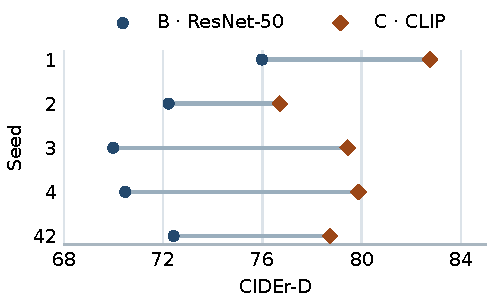
\includegraphics[width=\columnwidth]{figures/seed_comparison.pdf}
  \caption{CIDEr-D trên tập kiểm định theo năm seed trên Kaggle T4. Mỗi đường nối hai lượt chạy chung seed.}
  \label{fig:seeds}
\end{figure}

\begin{figure*}[t]
  \centering
  \begin{tabular}{@{}c@{\hspace{0.018\textwidth}}c@{\hspace{0.035\textwidth}}c@{\hspace{0.018\textwidth}}c@{}}
    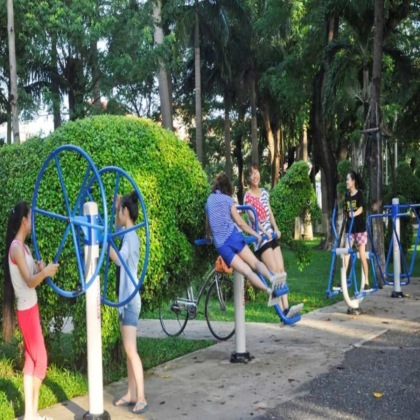
\includegraphics[width=.216\textwidth]{figures/scene_3091.jpg} &
    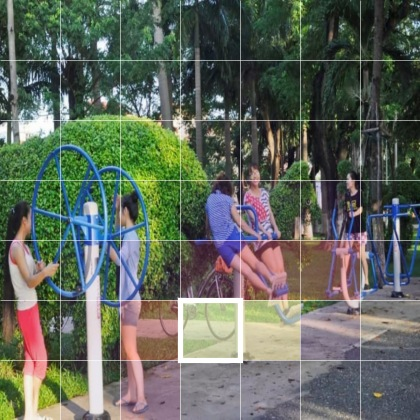
\includegraphics[width=.216\textwidth]{figures/attention_3091.jpg} &
    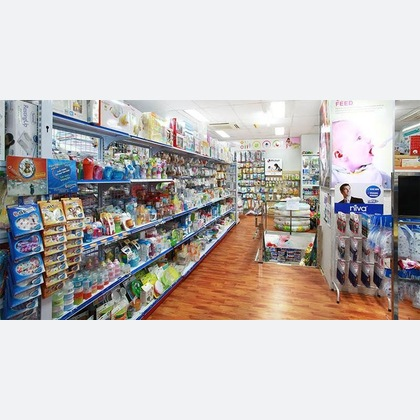
\includegraphics[width=.216\textwidth]{figures/scene_297.jpg} &
    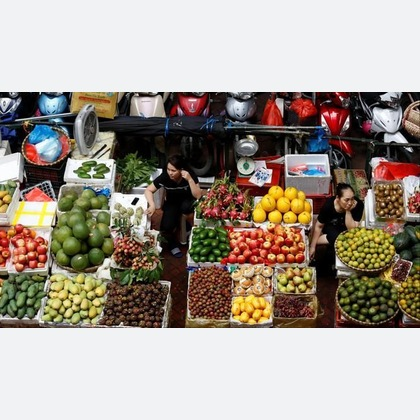
\includegraphics[width=.216\textwidth]{figures/scene_4568.jpg} \\
    \small (a) Ảnh 3091 &
    \small (b) Khi sinh “chụp” &
    \small (c) Ảnh đúng, hạng 392 &
    \small (d) Kết quả hạng 1
  \end{tabular}
  \caption{Ảnh test KTVIC và hai ca phân tích lỗi. (a--b) Ô viền trắng là vùng có trọng số cao nhất của A tại token “chụp”. (c--d) Hai kết quả từ chỉ mục B cho truy vấn về hàng hóa trên kệ: ảnh đúng có ID 297, còn ảnh 4568 đứng đầu.}
  \label{fig:cases}
\end{figure*}

\subsection{Lỗi chú thích và attention}

Tập phân tích có 40 ảnh test, ba cấu hình \modelA{}, \modelB{}, \modelAz{} và 120 câu. Hai lượt chấm xem 25 ảnh mỗi lượt, trong đó 10 ảnh trùng, với tên mô hình được ẩn. Mỗi câu nhận sáu cờ: sai vật thể, hành động, quan hệ, số lượng, chi tiết bịa hoặc lặp từ. Mỗi cờ có thể là $0$ (chưa thấy lỗi), $1$ (có lỗi) hoặc \texttt{?} (chưa rõ). Ở phần chung, 168/172 ô đã rõ trùng nhau trước khi đối chiếu (97,67\%). Tám ô còn lại chưa rõ ở cả hai lượt. Bốn bất đồng được rà lại dựa trên ảnh trước khi tổng hợp.

\begin{table}[t]
  \centering
  \begin{tabular}{lrrr}
    \toprule
    Loại lỗi & \modelA{} & \modelAz{} & \modelB{} \\
    \midrule
    Vật thể              & 7/37  & 9/36  & 10/38 \\
    Hành động            & 5/36  & 3/34  & 6/38 \\
    Quan hệ              & 2/38  & 2/39  & 7/38 \\
    Số lượng             & 0/40  & 1/40  & 0/40 \\
    Chi tiết bịa         & 11/40 & 8/40  & 6/39 \\
    Lặp từ               & 0/40  & 0/40  & 1/40 \\
    \midrule
    Có ít nhất một lỗi   & 20/34 & 23/33 & 24/34 \\
    \bottomrule
  \end{tabular}
  \caption{Số câu có lỗi trên số câu có nhãn đã rõ, tối đa 40 câu mỗi cấu hình. Hàng cuối tính là lỗi nếu có ít nhất một cờ 1, và chỉ tính là sạch nếu cả sáu cờ đều bằng 0.}
  \label{tab:errors}
\end{table}

Trong mẫu này, \modelB{} có nhiều câu sai quan hệ hơn \modelA{} (7/38 so với 2/38). \modelA{} lại có số câu bịa chi tiết cao nhất (11/40). Các cờ có thể đồng thời xuất hiện trên một câu, vì vậy tổng từng loại có thể lớn hơn số câu có lỗi. Bảng~\ref{tab:errors} mô tả mẫu đã xem, với quy trình chấm có AI hỗ trợ.

\subsection{Các ca minh họa}
\label{sec:cases}

\paragraph{Gọi sai hành động.}
Ảnh 3091 cho thấy một nhóm người dùng dụng cụ tập thể dục. \modelA{} sinh “có một nhóm người đang chụp ảnh tập thể dục ở trên đường”. \modelAz{} cũng sinh cụm “chụp ảnh”. Khi \modelA{} sinh “chụp”, ô gần bánh xe đạp và nền đường nhận trọng số cao nhất (11,05\%, hàng 6, cột 4 tính từ 1). A0 gán đều 2,04\% mỗi ô. Hình~\ref{fig:cases}a--b biểu diễn cách phân bố trọng số tại bước đó. Căn cứ để gán lỗi là nội dung câu và ảnh.

\paragraph{Tìm sai khi câu sinh thiếu từ khóa.}
Truy vấn “có nhiều loại hàng hoá được bày ra trên các kệ hàng” có đáp án ID 297. \modelB{} sinh “có một vài người đang đứng ở bên trong siêu thị”, nên câu sinh của ảnh đúng chỉ chia sẻ token “có” với truy vấn và đạt cosine 0,0134. Câu sinh của ảnh 4568 nói quả được bày trên kệ hàng và đạt 0,6941. Riêng “kệ” và “hàng” đóng góp khoảng 0,1997 vào điểm của ảnh đứng đầu. Hình~\ref{fig:cases}c--d minh họa sự khác biệt giữa nội dung ảnh và tín hiệu dùng để xếp hạng.

\paragraph{Tìm đúng và trường hợp hòa điểm.}
Với câu “đây là một bức ảnh chụp một tấm bản đồ”, chỉ mục \modelA{} trả đúng ảnh 5546 ở hạng 1 vì câu sinh giữ cụm “tấm bản đồ”. Với truy vấn về hàng hóa trên kệ, có bảy ảnh cùng chú thích và cùng cosine 0,8789 trong chỉ mục \modelA{}. Ảnh gốc 8678 đứng hạng 7 theo ID. Trong nhóm hòa điểm có những ảnh khác cũng phù hợp với mô tả.

\subsection{Điểm chú thích và điểm tìm ảnh}

Theo Bảng~\ref{tab:test}, \modelA{} tìm đúng 360/2.790 truy vấn ở top 5, so với 286 của \modelB{}. Chênh lệch là 2,65 điểm phần trăm (khoảng tin cậy 95\% từ 0,25 đến 4,84). \modelAz{} đạt 369 lượt, cao hơn \modelA{} chín lượt. Khoảng tin cậy 95\% của chênh lệch \modelAz{} trừ \modelA{} là từ $-1{,}97$ đến $2{,}62$ điểm phần trăm. \modelC{} có hạng trung vị tốt nhất (68), nhưng 308 lượt trúng top 5, thấp hơn cả hai cấu hình LSTM. BLEU và CIDEr-D đo độ khớp giữa câu sinh và tham chiếu cùng ảnh. Recall còn phụ thuộc liệu những từ khớp có giúp phân biệt ảnh gốc với các ảnh khác trong kho hay không.
